
\usetikzlibrary{positioning, arrows.meta, shapes.geometric, fit, backgrounds}
%\subsubsection{Diagrama de Flujo de Información}
\begin{figure}[H]
\centering
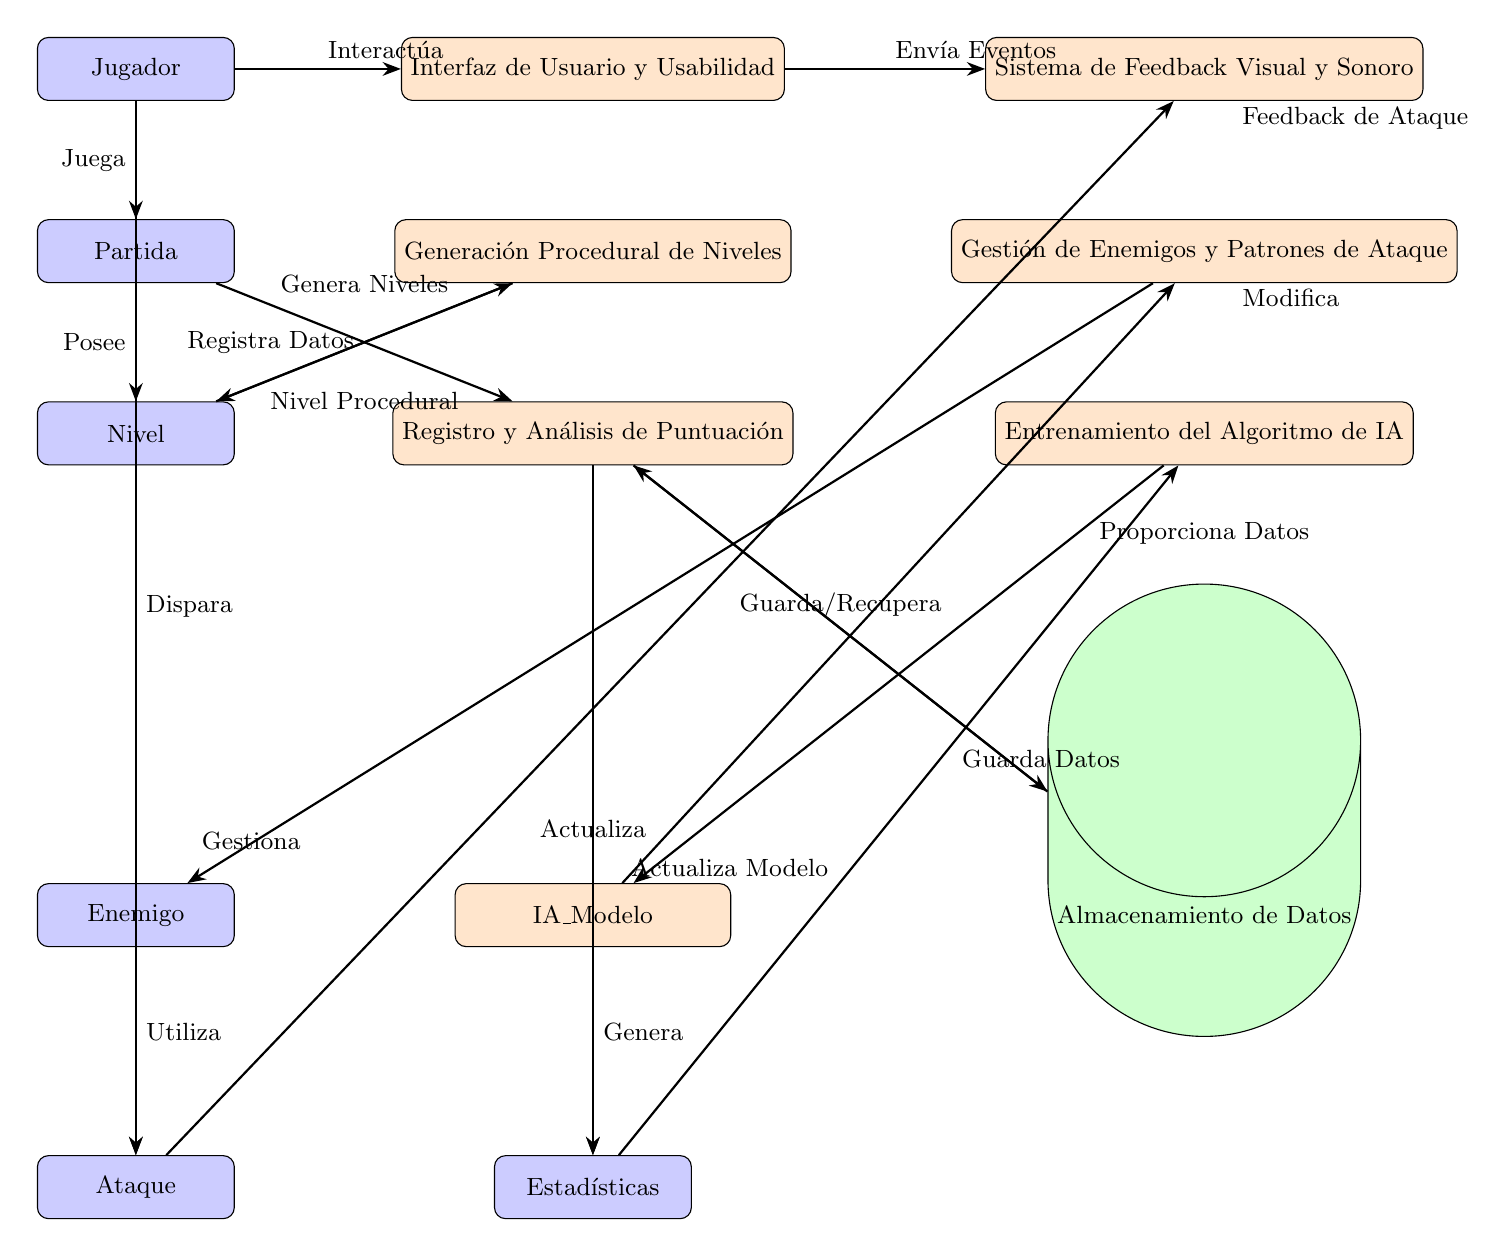
\begin{tikzpicture}[
    entity/.style={rectangle, draw, rounded corners, fill=blue!20, minimum width=2.5cm, minimum height=0.8cm, text centered, font=\small},
    process/.style={rectangle, draw, rounded corners, fill=orange!20, minimum width=3.5cm, minimum height=0.8cm, text centered, font=\small},
    data/.style={cylinder, shape border rotate=90, draw, fill=green!20, minimum width=2cm, minimum height=0.8cm, text centered, font=\small},
    arrow/.style={-{Stealth[scale=1]}, thick},
    every node/.style={font=\small},
    layer/.style={rectangle, draw=none, fill=none}
    ]

    % Definición de Capas
    \matrix[layer, column sep=2cm, row sep=1.5cm]{
        % Primera Columna: Entidades
        \node[entity] (Jugador) {Jugador}; &
        % Segunda Columna: Procesos
        \node[process] (Interfaz) {Interfaz de Usuario y Usabilidad}; &
        \node[process] (Feedback) {Sistema de Feedback Visual y Sonoro}; \\
        \node[entity] (Partida) {Partida}; &
        \node[process] (Generacion) {Generación Procedural de Niveles}; &
        \node[process] (GestionEnemigos) {Gestión de Enemigos y Patrones de Ataque}; \\
        \node[entity] (Nivel) {Nivel}; &
        \node[process] (Registro) {Registro y Análisis de Puntuación}; &
        \node[process] (EntrenamientoIA) {Entrenamiento del Algoritmo de IA}; \\
        \node[entity] (Enemigo) {Enemigo}; &
        \node[process] (IA_Modelo) {IA\_Modelo}; &
        \node[data] (Almacen) {Almacenamiento de Datos}; \\
        \node[entity] (Ataque) {Ataque}; &
        \node[entity] (Estadisticas) {Estadísticas}; &
        \\
    };

    % Conexiones entre Entidades y Procesos
    \draw[arrow] (Jugador) -- (Interfaz) node[midway, above right]{Interactúa};
    \draw[arrow] (Interfaz) -- (Feedback) node[midway, above right]{Envía Eventos};
    \draw[arrow] (Jugador) -- (Partida) node[midway, left]{Juega};
    \draw[arrow] (Partida) -- (Nivel) node[midway, left]{Posee};
    \draw[arrow] (Nivel) -- (Generacion) node[midway, above=.5cm]{Genera Niveles};
    \draw[arrow] (Generacion) -- (Nivel) node[midway, below=.5cm]{Nivel Procedural};
    \draw[arrow] (Partida) -- (Registro) node[midway, left]{Registra Datos};
    \draw[arrow] (Registro) -- (Estadisticas) node[midway, below]{Actualiza};
    \draw[arrow] (Estadisticas) -- (EntrenamientoIA) node[right, below=1cm]{Proporciona Datos};
    \draw[arrow] (EntrenamientoIA) -- (IA_Modelo) node[right, above right=0.5cm]{Actualiza Modelo};
    \draw[arrow] (IA_Modelo) -- (GestionEnemigos) node[right, below right=.5cm]{Modifica};
    \draw[arrow] (GestionEnemigos) -- (Enemigo) node[left,above right=1cm ]{Gestiona};
    \draw[arrow] (Jugador) -- (Ataque) node[midway, above right]{Dispara};
    \draw[arrow] (Enemigo) -- (Ataque) node[midway, above right]{Utiliza};
    \draw[arrow] (Ataque) -- (Feedback) node[right, below right=.5cm]{Feedback de Ataque};
    \draw[arrow] (IA_Modelo) -- (Estadisticas) node[midway, above right]{Genera};
    \draw[arrow] (Almacen) -- (Registro) node[midway, above]{Guarda/Recupera};
    \draw[arrow] (Registro) -- (Almacen) node[midway=2cm, below right=2cm]{Guarda Datos};

    % Ajustes adicionales para evitar solapamientos

\end{tikzpicture}
\caption{Diagrama de Flujo de Información del Proyecto}
\end{figure}
